\documentclass[tikz,fontsize=8pt]{standalone}
\usepackage{fourier}
\usetikzlibrary{arrows.meta}
\usetikzlibrary{calc}
\tikzset{>=latex}
\definecolor{bookblue}{RGB}{0,173,239}
\definecolor{bookpink}{RGB}{236,0,140}
\definecolor{bookgreen}{RGB}{50,200,0}
\definecolor{bookbluearea}{RGB}{204,239,252}
\tikzstyle{blueline}=[draw=bookblue,line width=0.2mm]
\tikzstyle{pinkline}=[draw=bookpink,line width=0.2mm]
\tikzstyle{greenline}=[draw=bookgreen,line width=0.2mm]
\tikzstyle{blackline}=[draw=black,line width=0.2mm]
\tikzstyle{bluearea}=[fill=bookbluearea]

\usepackage{scrextend}
\changefontsizes[8pt]{8pt}
\usetikzlibrary{decorations.pathreplacing}
\usetikzlibrary{shapes.misc, positioning}
\begin{document}
  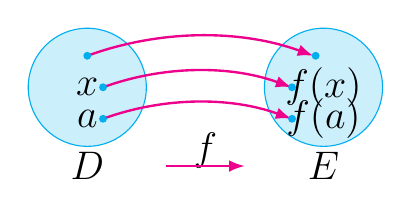
\begin{tikzpicture}
  \draw[fill=bookbluearea,draw=bookblue] (0,0) ellipse (0.75cm and 0.75cm);
  \draw[fill=bookbluearea,draw=bookblue] (3,0) ellipse (0.75cm and 0.75cm);
  \node at (0,0) {\Large $x$};
  \node at (0,-0.4) {\Large $a$};
  \node at (3,0) {\Large $f(x)$};
  \node at (3,-0.4) {\Large $f(a)$};
  \draw[bookpink,-{Latex[length=2mm]},line width=0.3mm] (0.2,0) arc (110:70:3.5cm);
  \draw[bookpink,-{Latex[length=2mm]},line width=0.3mm] (0.2,-0.4) arc (110:70:3.5cm);
  \draw[bookpink,-{Latex[length=2mm]},line width=0.3mm] (0,0.4) arc (110:70:4.2cm);
  \fill[bookblue] (0.2,0) circle (0.5mm);
  \fill[bookblue] (0.2,-0.4) circle (0.5mm);
  \fill[bookblue] (0, 0.4) circle (0.5mm);
  
  \fill[bookblue] (2.6,0) circle (0.5mm);
  \fill[bookblue] (2.6,-0.4) circle (0.5mm);
  \fill[bookblue] (2.9, 0.4) circle (0.5mm);
  
  \node at (0,-1) {\Large $D$};
  \node at (3,-1) {\Large $E$};
  \node at (1.5,-0.8) {\Large $f$};
  \draw[bookpink,-{Latex[length=2mm]}, line width=0.3mm] (1,-1) -- (2,-1);
  
  %\draw [bookblue, fill=bookbluearea] plot [smooth cycle, tension=1] coordinates {(-0.1,0) (-0.3,1) (0.5,1) (0.9,0) (0.5,-1) (-0.3,-1)};
  %\node (1) [draw=bookblue,fill=bookbluearea,draw, rounded corners=1mm, minimum width=0.7cm, minimum height=0.6cm] {$f$};
  %\path[draw=bookpink, ->] (-1.2,0) -- (-0.35,0);
  %\path[draw=bookpink, ->] (0.35,0) -- (1.2,0);
  %\node at (-0.8,-0.2) {\footnotesize entrada};
  %\node at (0.75,-0.2) {\footnotesize saida};
  %\node at (-0.8,0.18) {\footnotesize $x$};
  %\node at (0.75,0.18) {\footnotesize $y=f(x)$};
%  \node at (-0.15,-0.2) {0};
%  \draw[->] (-0.5,0) -- (2.3,0) node[below] {$x$};
%  \draw[->] (0,-0.5) -- (0,2.3) node[left] {$y$};
%  
%  \draw[blackline,domain=-1.1:0.5] plot (\x+1.5,{-(\x)^2+1.5});
%  \draw[pinkline] (0.256,0.15) -- (1.356,1.91);
%  \fill (0.68,0.83) circle (0.4mm);
%  \node at (0.5,0.83) {$P$};
%  \node at (1.2,2) {$t$};
%  \node at (1.7,1) {$y=f(x)$};
  \end{tikzpicture}
\end{document}